\documentclass[aspectratio=169,9pt,t]{beamer}

\usepackage[T1]{fontenc}
\usepackage{lmodern}
\usepackage{amsmath,amssymb,mathtools}
\usepackage{booktabs,tabularx,array}
\usepackage{tikz}
\usetikzlibrary{arrows.meta,positioning,calc,fit,shapes.geometric,decorations.pathreplacing}
\pdfstringdefDisableCommands{\def\translate#1{#1}}

% ---------- palette and Beamer setup ----------
\definecolor{Ink}{HTML}{172033}
\definecolor{Muted}{HTML}{5F6B7A}
\definecolor{Canvas}{HTML}{FAFAF7}
\definecolor{Graph}{HTML}{6B7280}
\definecolor{BP}{HTML}{1769AA}
\definecolor{BPSoft}{HTML}{E8F2FA}
\definecolor{GD}{HTML}{C65D21}
\definecolor{GDSoft}{HTML}{FCEFE7}
\definecolor{Tied}{HTML}{A26400}
\definecolor{TiedSoft}{HTML}{FFF3D6}
\definecolor{Good}{HTML}{16794A}
\definecolor{GoodSoft}{HTML}{E7F6EE}
\definecolor{Bad}{HTML}{B42318}
\definecolor{BadSoft}{HTML}{FDECEA}

\usetheme{default}
\usefonttheme{professionalfonts}
\setbeamertemplate{navigation symbols}{}
\setbeamercolor{normal text}{fg=Ink,bg=Canvas}
\setbeamercolor{frametitle}{fg=Ink,bg=Canvas}
\setbeamercolor{title}{fg=Ink}
\setbeamercolor{subtitle}{fg=Muted}
\setbeamercolor{alerted text}{fg=Bad}
\setbeamersize{text margin left=7mm,text margin right=7mm}
\setbeamertemplate{itemize item}{\color{BP}$\blacktriangleright$}
\setbeamertemplate{itemize subitem}{\color{Graph}$\bullet$}
\setbeamertemplate{enumerate item}{\color{BP}\insertenumlabel.}
\setbeamertemplate{frametitle}{%
  \vspace{1.2mm}\insertframetitle\par
  \vspace{0.5mm}{\color{Graph}\rule{\textwidth}{0.45pt}}\vspace{-1.5mm}}
\setbeamertemplate{footline}{%
  \leavevmode\hbox{%
    \begin{beamercolorbox}[wd=.84\paperwidth,ht=2.7ex,dp=1.2ex,leftskip=7mm]{normal text}%
      \scriptsize\color{Muted}BP--GD mechanism study
    \end{beamercolorbox}%
    \begin{beamercolorbox}[wd=.16\paperwidth,ht=2.7ex,dp=1.2ex,rightskip=7mm plus 1fil]{normal text}%
      \scriptsize\color{Muted}\insertframenumber
    \end{beamercolorbox}}}

% ---------- reusable presentation elements ----------
\newcommand{\evidence}[1]{%
  \vfill\hfill{\fontsize{5.8}{6.8}\selectfont\color{Muted}Evidence: #1}}
\newcommand{\scopebox}[1]{%
  \begin{beamercolorbox}[rounded=true,sep=1.3ex]{block body}
    \small #1
  \end{beamercolorbox}}
\newcommand{\takeaway}[1]{%
  \begin{beamercolorbox}[rounded=true,sep=1.5ex]{title}
    \centering\normalsize\bfseries #1
  \end{beamercolorbox}}
\newcommand{\BPtag}[1]{\tikz[baseline=(x.base)]\node[fill=BPSoft,draw=BP,rounded corners=2pt,inner xsep=4pt,inner ysep=2pt,text=BP] (x) {#1};}
\newcommand{\GDtag}[1]{\tikz[baseline=(x.base)]\node[fill=GDSoft,draw=GD,dashed,rounded corners=2pt,inner xsep=4pt,inner ysep=2pt,text=GD] (x) {#1};}
\newcommand{\goodtag}[1]{\tikz[baseline=(x.base)]\node[fill=GoodSoft,draw=Good,rounded corners=2pt,inner xsep=5pt,inner ysep=2pt,text=Good] (x) {#1};}
\newcommand{\badtag}[1]{\tikz[baseline=(x.base)]\node[fill=BadSoft,draw=Bad,rounded corners=2pt,inner xsep=5pt,inner ysep=2pt,text=Bad] (x) {#1};}

\tikzset{
  bit/.style={circle,draw=Graph,fill=white,line width=.8pt,minimum size=8mm,inner sep=0pt,font=\small},
  check/.style={rectangle,draw=Graph,fill=white,line width=.8pt,minimum size=7.5mm,inner sep=0pt,font=\small},
  edge/.style={draw=Graph!62,line width=1.15pt},
  bpedge/.style={draw=BP,line width=2.3pt,-{Stealth[length=2.3mm]}},
  gdedge/.style={draw=GD,line width=2.3pt,dashed,-{Stealth[length=2.3mm]}},
  process/.style={draw=Graph,fill=white,rounded corners=3pt,align=center,minimum height=9mm,inner xsep=4pt},
  bpbox/.style={draw=BP,fill=BPSoft,rounded corners=3pt,align=center,inner sep=5pt},
  gdbox/.style={draw=GD,fill=GDSoft,dashed,rounded corners=3pt,align=center,inner sep=5pt},
  tiedbox/.style={draw=Tied,fill=TiedSoft,rounded corners=3pt,align=center,inner sep=5pt},
  goodbox/.style={draw=Good,fill=GoodSoft,rounded corners=3pt,align=center,inner sep=5pt},
  badbox/.style={draw=Bad,fill=BadSoft,rounded corners=3pt,align=center,inner sep=5pt}
}

\newcommand{\chainbase}[1]{%
  \node[bit] (#1b1) at (0,0) {$b_1$};
  \node[check] (#1A) at (1.5,0) {$A$};
  \node[bit] (#1b2) at (3.0,0) {$b_2$};
  \node[check] (#1B) at (4.5,0) {$B$};
  \node[bit] (#1b3) at (6.0,0) {$b_3$};
  \draw[edge] (#1b1)--(#1A)--(#1b2)--(#1B)--(#1b3);
}

\title{Same Tanner Graph, Different State}
\subtitle{Why Tanner-graph traversal is not a sufficient mechanism}
\author{}
\date{Evidence through 28 October 2026}

\begin{document}

% 1
\begin{frame}[plain]
  \vspace{5mm}
  {\usebeamerfont{title}\color{Ink}\LARGE\bfseries\inserttitle\par}
  \vspace{2mm}
  {\usebeamerfont{subtitle}\color{Muted}\large\insertsubtitle\par}

  \vspace{7mm}
  \centering
  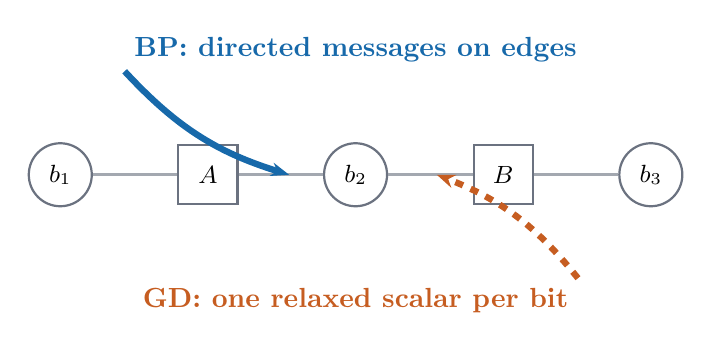
\begin{tikzpicture}[x=1.25cm,y=1cm]
    \chainbase{t}
    \node[above=9mm of tb2,text=BP,font=\bfseries] (bp) {BP: directed messages on edges};
    \node[below=9mm of tb2,text=GD,font=\bfseries] (gd) {GD: one relaxed scalar per bit};
    \draw[bpedge] (bp.south west) to[bend right=15] ($(tA)!0.55!(tb2)$);
    \draw[gdedge] (gd.north east) to[bend right=15] ($(tb2)!0.55!(tB)$);
  \end{tikzpicture}

  \vspace{6mm}
  \takeaway{The graph specifies who is connected. It does not specify what is represented, retained, or used to calculate the next state.}

  \vfill
  {\scriptsize\color{Muted}Research question: what mechanism, or combination of mechanisms, differentiates BP from projected gradient descent?}
\end{frame}

% 2
\begin{frame}{A performance ordering cannot identify the mechanism}
  \centering
  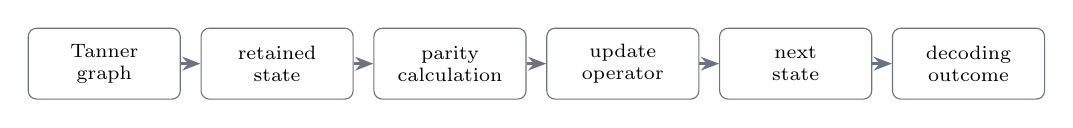
\begin{tikzpicture}[node distance=2.5mm,>=Stealth,font=\scriptsize]
    \node[process,text width=1.65cm] (graph) {Tanner\\graph};
    \node[process,text width=1.65cm,right=of graph] (state) {retained\\state};
    \node[process,text width=1.65cm,right=of state] (parity) {parity\\calculation};
    \node[process,text width=1.65cm,right=of parity] (update) {update\\operator};
    \node[process,text width=1.65cm,right=of update] (next) {next\\state};
    \node[process,text width=1.65cm,right=of next] (outcome) {decoding\\outcome};
    \foreach \a/\b in {graph/state,state/parity,parity/update,update/next,next/outcome}
      \draw[-{Stealth[length=2.3mm]},line width=1.1pt,draw=Graph] (\a)--(\b);
  \end{tikzpicture}

  \vspace{5mm}
  \begin{columns}[T,onlytextwidth]
    \column{.64\textwidth}
      \scopebox{A native BP--GD comparison changes several boxes at once. It can show that the methods behave differently, but it cannot say which box caused the difference.}
    \column{.32\textwidth}
      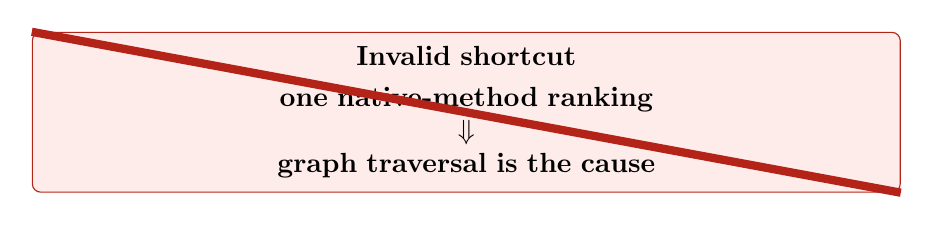
\begin{tikzpicture}
        \node[badbox,text width=.88\linewidth] (shortcut) {\bfseries Invalid shortcut\\[1mm]
          one native-method ranking\\$\Downarrow$\\graph traversal is the cause};
        \draw[Bad,line width=3pt] (shortcut.north west)--(shortcut.south east);
      \end{tikzpicture}
  \end{columns}

  \vspace{3mm}
  \takeaway{We need a controlled change, not an explanation inferred from the final ranking.}
  \evidence{RQ1-ENDPOINT-001 experiment card; mechanism report, lines 7--28}
\end{frame}

% 3
\begin{frame}{Both methods use the same Tanner-graph edges}
  \centering
  \begin{tikzpicture}[x=1.27cm,y=1cm]
    \node[anchor=east,text=BP,font=\bfseries] at (-.35,.9) {BP};
    \begin{scope}[yshift=.9cm]\chainbase{p}\end{scope}
    \node[anchor=east,text=GD,font=\bfseries] at (-.35,-.9) {GD};
    \begin{scope}[yshift=-.9cm]\chainbase{g}\end{scope}

    \only<2>{
      \begin{scope}[overlay]
      \draw[BP,line width=3pt] (pb1)--(pA)--(pb2);
      \draw[GD,line width=3pt,dashed] (gb1)--(gA)--(gb2);
      \end{scope}
    }
    \only<3>{
      \begin{scope}[overlay]
      \draw[BP,line width=3pt] (pb2)--(pB)--(pb3);
      \draw[GD,line width=3pt,dashed] (gb2)--(gB)--(gb3);
      \end{scope}
    }
  \end{tikzpicture}

  \vspace{1mm}
  \begin{columns}[T,onlytextwidth]
    \column{.48\textwidth}
    \begin{beamercolorbox}[rounded=true,sep=1.2ex]{normal text}
      \textcolor{BP}{\bfseries BP} forms variable-to-check and check-to-variable messages on directed edges.
    \end{beamercolorbox}
    \column{.48\textwidth}
    \begin{beamercolorbox}[rounded=true,sep=1.2ex]{normal text}
      \textcolor{GD}{\bfseries Projected GD} uses neighbouring scalar values when evaluating partial derivatives of its objective function.
    \end{beamercolorbox}
  \end{columns}

  \vspace{1mm}
  \takeaway{The Tanner graph organizes both calculations; GD does not need a separate ``gradient graph.''}
  \evidence{mailboxes\_and\_arrows.html; mechanism report, lines 313--322}
\end{frame}

% 4
\begin{frame}{BP: the recipient determines the message}
  \begin{columns}[T,onlytextwidth]
    \column{.54\textwidth}
    \centering
    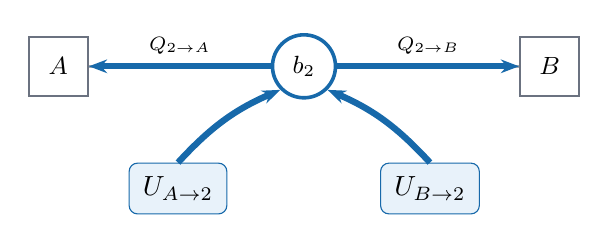
\begin{tikzpicture}[x=1.2cm,y=1cm]
      \node[check] (A) at (0,1.3) {$A$};
      \node[bit,draw=BP,line width=1.3pt] (b2) at (2.6,1.3) {$b_2$};
      \node[check] (B) at (5.2,1.3) {$B$};
      \draw[edge] (A)--(b2)--(B);
      \node[bpbox,below=8mm of b2,xshift=-16mm] (UA) {$U_{A\to2}$};
      \node[bpbox,below=8mm of b2,xshift=16mm] (UB) {$U_{B\to2}$};
      \draw[bpedge] (UA.north) to[bend left=12] (b2.south west);
      \draw[bpedge] (UB.north) to[bend right=12] (b2.south east);
      \draw[bpedge] (b2) -- node[above,font=\scriptsize] {$Q_{2\to A}$} (A);
      \draw[bpedge] (b2) -- node[above,font=\scriptsize] {$Q_{2\to B}$} (B);
    \end{tikzpicture}

    \column{.44\textwidth}
    \vspace{4mm}
    \begin{align*}
      Q_{2\to A} &= L_2 + U_{B\to2},\\
      Q_{2\to B} &= L_2 + U_{A\to2}.
    \end{align*}
    {\scriptsize\color{Muted}Sign convention:
      $L_i=\log\!\frac{P(b_i=1\mid y_i)}{P(b_i=0\mid y_i)}$; positive $L_i$ favors bit one.}
    \begin{itemize}
      \item The message to $A$ omits the preceding message from $A$.
      \item The message to $B$ omits the preceding message from $B$.
      \item One bit can therefore send different values to different checks.
    \end{itemize}
  \end{columns}

  \vspace{2mm}
  \takeaway{BP augments each Tanner-graph edge with separately addressed directed message coordinates.}
  \evidence{RQ1-STATE-002; mechanism report, lines 44--65}
\end{frame}

% 5
\begin{frame}{Projected GD: one scalar state per bit}
  \begin{columns}[T,onlytextwidth]
    \column{.52\textwidth}
    \centering
    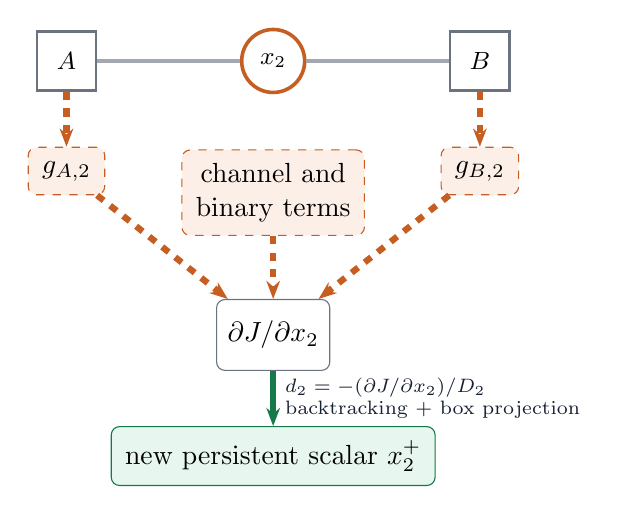
\begin{tikzpicture}[x=1.05cm,y=1cm]
      \node[check] (A) at (0,1.5) {$A$};
      \node[bit,draw=GD,line width=1.3pt] (b2) at (2.5,1.5) {$x_2$};
      \node[check] (B) at (5,1.5) {$B$};
      \draw[edge] (A)--(b2)--(B);
      \node[gdbox,below=7mm of A] (gA) {$g_{A,2}$};
      \node[gdbox,below=7mm of B] (gB) {$g_{B,2}$};
      \node[gdbox,below=7mm of b2] (local) {channel and\\binary terms};
      \node[process,below=8mm of local] (sum) {$\partial J/\partial x_2$};
      \node[goodbox,below=7mm of sum] (newx) {new persistent scalar $x_2^+$};
      \draw[gdedge] (A)--(gA);
      \draw[gdedge] (B)--(gB);
      \draw[gdedge] (gA)--(sum);
      \draw[gdedge] (gB)--(sum);
      \draw[gdedge] (local)--(sum);
      \draw[-{Stealth[length=2.3mm]},draw=Good,line width=2pt] (sum)--
        node[right,font=\scriptsize,text=Ink,align=left]{$d_2=-(\partial J/\partial x_2)/D_2$\\backtracking + box projection}(newx);
    \end{tikzpicture}

    \column{.46\textwidth}
    \small
    {\scriptsize\color{Muted}Native coordinate: $\boldsymbol\ell=-\mathbf L$ and
      $x_i>0$ represents bit zero; $D_i=(2\mu_p\deg(i)+8\mu_b)/n$.}\par\vspace{-1mm}
    \begin{align*}
      J(\mathbf{x})={}&-\frac{\boldsymbol\ell^{\mathsf T}\mathbf{x}}{2n}
      +\frac{\mu_p}{n}\sum_c\left(1-\prod_{j\in\mathcal N(c)}x_j\right)^2\\
      &+\frac{\mu_b}{n}\sum_i(1-x_i^2)^2,\\[1mm]
      \frac{\partial J}{\partial x_2}={}&g_{A,2}+g_{B,2}
        +g_{\mathrm{ch},2}+g_{\mathrm{bin},2}.
    \end{align*}
    \begin{itemize}
      \item All terms use the same frozen $\mathbf{x}$ and are combined for this update.
      \item Only the accepted projected $x_2^+$ enters the next update.
    \end{itemize}
  \end{columns}

  \begin{beamercolorbox}[rounded=true,sep=.8ex]{block body}
    \footnotesize The quantities $g_{A,2}$ and $g_{B,2}$ contribute to a partial derivative of the objective function. They are not BP messages, and their summation is the declared operation for this scalar objective.
  \end{beamercolorbox}
  \evidence{RQ1-ENDPOINT-PG-001 method description and validated native trace}
\end{frame}

% 6
\begin{frame}{The decisive visual: what crosses the iteration boundary?}
  \centering
  \begin{tikzpicture}[x=1cm,y=1cm]
    \path[use as bounding box] (-5.6,-2.25) rectangle (5.8,2.35);
    \draw[Graph,line width=1.1pt,dashed] (0,2.25)--(0,-2.1);
    \node[rotate=90,fill=Canvas,inner sep=2pt,text=Muted,font=\small\bfseries] at (0,.1) {iteration boundary};
    \node[anchor=west,text=Muted,font=\scriptsize,fill=Canvas,inner sep=1pt] at (-5.35,2.08) {boundaries shown: after the BP check update / accepted GD update};

    \node[anchor=east,text=BP,font=\bfseries] at (-5.3,1.3) {BP};
    \node[bpbox] (ua) at (-3.7,1.65) {$U_{A\to2}$};
    \node[bpbox] (ub) at (-3.7,.85) {$U_{B\to2}$};
    \node[bpbox] (ua2) at (3.1,1.65) {$U_{A\to2}$};
    \node[bpbox] (ub2) at (3.1,.85) {$U_{B\to2}$};
    \draw[bpedge] (ua)--(ua2);
    \draw[bpedge] (ub)--(ub2);
    \node[anchor=west,text=BP,font=\small\bfseries] at (4.2,1.25) {both remain separate};

    \node[anchor=east,text=GD,font=\bfseries] at (-5.3,-.65) {GD};
    \node[gdbox] (ga) at (-4,-.35) {$g_{A,2}$};
    \node[gdbox] (gb) at (-4,-1.05) {$g_{B,2}$};
    \node[process] (add) at (-1.45,-.7) {sum + accepted\\update};
    \node[goodbox] (xnew) at (3.1,-.7) {$x_2^+$};
    \draw[gdedge] (ga)--(add);
    \draw[gdedge] (gb)--(add);
    \draw[-{Stealth[length=2.3mm]},draw=Good,line width=2.3pt] (add)--(xnew);

    \only<1>{
      \begin{scope}[overlay]
      \node[below=3mm of add,text=GD,font=\small] {temporary calculations are still visible};
      \end{scope}
    }
    \only<2->{
      \begin{scope}[overlay]
      \fill[Canvas,opacity=.88] (-5,-1.45) rectangle (-.1,.05);
      \node[text=Muted,font=\small,align=center] at (-2.8,-.7) {partial-derivative\\terms are not retained separately};
      \end{scope}
    }
    \only<3>{
      \begin{scope}[overlay]
      \node[goodbox,text width=10cm,font=\small] at (0,-1.83) {\bfseries When the graph is revisited, BP retains separately addressed $U_{A\to2}$ and $U_{B\to2}$, then forms recipient-excluding $Q$ messages; GD retains one updated $x_2$.};
      \end{scope}
    }
  \end{tikzpicture}

  \evidence{mailboxes\_and\_arrows.html, beats 19--20; RQ1 endpoint method description}
\end{frame}

% 7
\begin{frame}{Iteration 2 revisits the same edges with different information}
  \begin{columns}[T,onlytextwidth]
    \column{.49\textwidth}
    \begin{beamercolorbox}[rounded=true,sep=1.1ex]{normal text}
      \centering\textcolor{BP}{\large\bfseries BP}\par\vspace{2mm}
      \begin{align*}
        Q_{2\to A}&=L_2+U_{B\to2},\\
        Q_{2\to B}&=L_2+U_{A\to2}.
      \end{align*}
      \BPtag{$A$ receives $Q_{2\to A}$}\qquad
      \BPtag{$B$ receives $Q_{2\to B}$}

      \vspace{3mm}
      The two values can differ because they use different separately retained incoming $U$ messages.
    \end{beamercolorbox}

    \column{.49\textwidth}
    \begin{beamercolorbox}[rounded=true,sep=1.1ex]{normal text}
      \centering\textcolor{GD}{\large\bfseries Projected GD}\par\vspace{2mm}
      \[
        \text{check }A\text{ reads }x_2^+,
        \qquad
        \text{check }B\text{ reads }x_2^+.
      \]

      \GDtag{$A$ reads $x_2^+$}\qquad
      \GDtag{$B$ reads $x_2^+$}

      \vspace{3mm}
      Any effect that remains after the objective terms are summed, the step is selected and the box projection is applied is available only through the updated scalar.
    \end{beamercolorbox}
  \end{columns}

  \vspace{3mm}
  \takeaway{The difference is not whether the graph is revisited. It is what information is available when it is revisited.}
  \evidence{RQ1-STATE-002; RQ1-ENDPOINT-001 validated native trace}
\end{frame}

% 8
\begin{frame}{Controlled test: remove only the recipient-specific distinction}
  \begin{columns}[T,onlytextwidth]
    \column{.55\textwidth}
    \begin{align*}
      Q^{\star}_{i\to a}
        &=L_i+\sum_{b\in\mathcal N(i)\setminus\{a\}}U_{b\to i},\\
      \bar q_i
        &=\operatorname{mean}_{a\in\mathcal N(i)}Q^{\star}_{i\to a},\\
      \delta_{i\to a}
        &=Q^{\star}_{i\to a}-\bar q_i.
    \end{align*}

    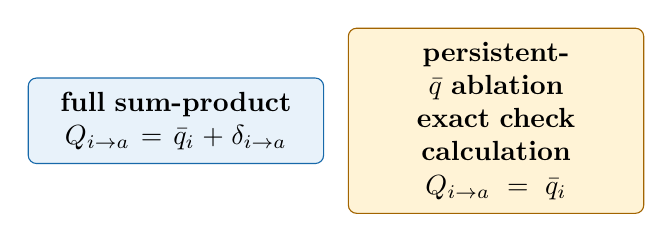
\begin{tikzpicture}[node distance=3mm]
      \node[bpbox,text width=3.4cm] (full) {\bfseries full sum-product\\$Q_{i\to a}=\bar q_i+\delta_{i\to a}$};
      \node[tiedbox,text width=3.4cm,right=of full] (tied) {\bfseries persistent-$\bar q$ ablation\\exact check calculation\\$Q_{i\to a}=\bar q_i$};
    \end{tikzpicture}

    \column{.42\textwidth}
    \scopebox{\textbf{Held fixed}
      \begin{itemize}
        \item parity-check matrix and Tanner graph;
        \item received samples and channel LLRs;
        \item exact check calculation;
        \item flooding schedule and initialization;
        \item stopping rule and 80-iteration limit;
        \item arrays remain indexed by Tanner-graph edge.
      \end{itemize}}
  \end{columns}

  \vspace{1mm}
  \begin{beamercolorbox}[rounded=true,sep=1.2ex]{alerted text}
    \centering\bfseries This is a controlled test inside exact sum-product BP. The ablation branch is not projected GD.
  \end{beamercolorbox}
  \evidence{RQ2-AWGN-001 experiment card, lines 24--64}
\end{frame}

% 9
\begin{frame}{Toy pulse: trajectories separate at the first possible point}
  \centering
  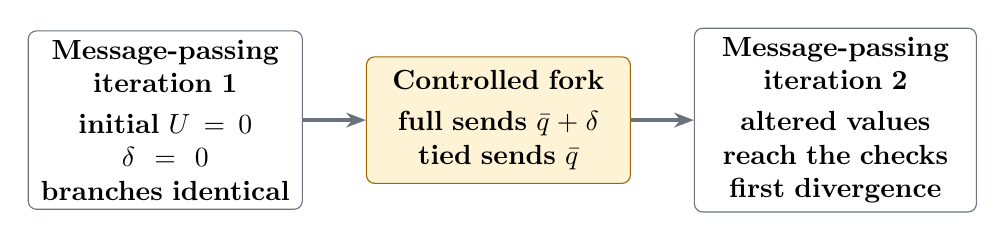
\begin{tikzpicture}[node distance=5mm and 8mm,>=Stealth]
    \node[process,text width=3.2cm] (i1) {\bfseries Message-passing iteration 1\\[1mm]
      initial $U=0$\\$\delta=0$\\branches identical};
    \node[tiedbox,text width=3.0cm,right=of i1] (fork) {\bfseries Controlled fork\\[1mm]
      full sends $\bar q+\delta$\\tied sends $\bar q$};
    \node[process,text width=3.3cm,right=of fork] (i2) {\bfseries Message-passing iteration 2\\[1mm]
      altered values reach the checks\\first divergence};
    \draw[-{Stealth[length=2.5mm]},draw=Graph,line width=1.5pt] (i1)--(fork);
    \draw[-{Stealth[length=2.5mm]},draw=Graph,line width=1.5pt] (fork)--(i2);
  \end{tikzpicture}

  \vspace{5mm}
  \begin{columns}[T,onlytextwidth]
    \column{.49\textwidth}
    \begin{beamercolorbox}[rounded=true,sep=1.3ex]{normal text}
      \centering\textcolor{BP}{\bfseries Full branch at the shared bit}
      \[
        Q^{\star}_{2\to A}=\ln 3,
        \qquad
        Q^{\star}_{2\to B}=\ln(1/6).
      \]
      \centering\goodtag{hard-decision estimate 000}\quad\goodtag{syndrome 00}
    \end{beamercolorbox}
    \column{.49\textwidth}
    \begin{beamercolorbox}[rounded=true,sep=1.3ex]{normal text}
      \centering\textcolor{Tied}{\bfseries Tied branch at the shared bit}
      \[
        Q_{2\to A}=Q_{2\to B}=-\tfrac12\ln 2.
      \]
      \centering\badtag{hard-decision estimate 001}\quad\badtag{syndrome 01}
    \end{beamercolorbox}
  \end{columns}

  \vspace{3mm}
  \scriptsize\centering Reconstructing $\bar q+\delta$ restores the full trajectory; on the degree-one six-bit graph, $\delta=0$ and tying is a null intervention.\\
  \textcolor{Muted}{This one-update snapshot may later rejoin full BP; it is not a convergence or performance result. The next slide is a separate persistent $N=10200$ ablation.}
  \evidence{RQ1-STATE-002; mechanism report, lines 127--185}
\end{frame}

% 10
\begin{frame}{The recipient-specific distinction changes recovery on locked AWGN frames}
  \begin{columns}[c,onlytextwidth]
    \column{.57\textwidth}
    \centering
    \renewcommand{\arraystretch}{1.35}
    \begin{tabular}{>{\raggedright\arraybackslash}p{4.1cm}cc}
      \toprule
      \textbf{Locked AWGN frames} & \textbf{Full} & \textbf{Persistent $\bar q$}\\
      \midrule
      Sealed descriptive anchor & \textcolor{Good}{\bfseries 24/24} & \textcolor{Bad}{\bfseries 0/24}\\
      Supporting 200-frame transfer & \textcolor{Good}{\bfseries 200/200} & \textcolor{Bad}{\bfseries 0/200}\\
      \bottomrule
    \end{tabular}

    \vspace{4mm}
    {\small The counts are the same for both registered endpoints: parity validity and equality to the transmitted word.\\[1mm]
      \scriptsize Regular $(3,6)$ LDPC, $N=10200$, all-zero word, $E_s/N_0=1.5$ dB, 80-message-passing-iteration cap.}

    \column{.39\textwidth}
    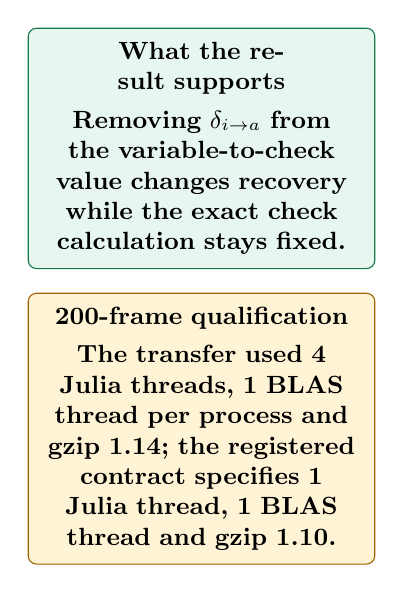
\begin{tikzpicture}
      \node[goodbox,text width=4.05cm,font=\small] (est) {\bfseries What the result supports\\[1mm]
        Removing $\delta_{i\to a}$ from the variable-to-check value changes recovery while the exact check calculation stays fixed.};
      \node[tiedbox,text width=4.05cm,font=\small,below=3mm of est] (caveat) {\bfseries 200-frame qualification\\[1mm]
        The transfer used 4 Julia threads, 1 BLAS thread per process and gzip 1.14; the registered contract specifies 1 Julia thread, 1 BLAS thread and gzip 1.10.};
    \end{tikzpicture}
  \end{columns}

  \vspace{1mm}
  \takeaway{The graph, flooding schedule, per-iteration check calculation and 80-iteration cap were fixed; removing $\delta_{i\to a}$ from $Q$ changed recovery. Realized iteration count was an outcome.}
  \evidence{RQ2-AWGN-001 anchor and valid parallel transfer; mechanism report, lines 249--305}
\end{frame}

% 11
\begin{frame}{The update operator also changes the trajectory after one update}
  \begin{columns}[T,onlytextwidth]
    \column{.48\textwidth}
    \begin{beamercolorbox}[rounded=true,sep=1.4ex]{normal text}
      \centering\textcolor{BP}{\large\bfseries Direct BP map}\par\vspace{2mm}
      \[
        \mathbf u^{+}=F_s(\mathbf u)
      \]
      The calculated check-to-variable state is assigned directly.
    \end{beamercolorbox}

    \column{.48\textwidth}
    \begin{beamercolorbox}[rounded=true,sep=1.4ex]{normal text}
      \centering\textcolor{Graph}{\large\bfseries BP-residual gradient control}\par\vspace{2mm}
      \[
        \mathbf u^{+}=\mathbf u-\alpha
        (I-J_s)^{\mathsf T}(\mathbf u-F_s(\mathbf u)).
      \]
      One gradient step is taken on
      $R_s(\mathbf u)=\tfrac12\lVert\mathbf u-F_s(\mathbf u)\rVert_2^2$,\\
      {\scriptsize where $J_s=\partial F_s(\mathbf u)/\partial\mathbf u$.}
    \end{beamercolorbox}
  \end{columns}

  \vspace{1mm}
  \begin{columns}[c,onlytextwidth]
    \column{.63\textwidth}
      \centering\scriptsize
      \renewcommand{\arraystretch}{1.25}
      \begin{tabular}{>{\bfseries}r|cc}
        & direct BP map & BP-residual gradient step\\
        \hline
        recipient-specific $Q$ & $(S,D)$ & $(S,G)$\\
        tied $Q=\bar q$ & $(T,D)$ & $(T,G)$
      \end{tabular}
    \column{.34\textwidth}
      \begin{beamercolorbox}[rounded=true,sep=1.1ex]{normal text}
        \centering\small After one update, the state, update and interaction vector contrasts are nonzero on the tree and cycle.
      \end{beamercolorbox}
  \end{columns}

  \vspace{0mm}
  \scopebox{This $2\times2$ control uses BP edge coordinates and the squared objective $R_s(\mathbf u)=\tfrac12\lVert\mathbf u-F_s(\mathbf u)\rVert_2^2$---not the native projected-GD decoder. It shows that the recipient-specific $Q$ calculation and next-state operator must be tested separately.}
  \evidence{RQ1-UPDATE-001 and RQ1-UPDATE-CYCLE-001}
\end{frame}

% 12
\begin{frame}{Current answer: what we know and what remains open}
  \begin{columns}[T,onlytextwidth]
    \column{.49\textwidth}
    \begin{beamercolorbox}[rounded=true,sep=1.2ex]{normal text}
      \small
      \textcolor{Good}{\large\bfseries Established}
      \begin{itemize}
        \item Within the controlled sum-product cases, Tanner-graph traversal alone is not a sufficient description.
        \item Recipient-specific variable-to-check information is causally important inside the tested recurrence.
        \item Discarding $\delta_{i\to a}$ from the variable-to-check value consumed by each check changed parity validity and equality to the transmitted word.
        \item A separate BP-coordinate control shows that the update operator also changes the trajectory after one update.
      \end{itemize}
    \end{beamercolorbox}

    \column{.49\textwidth}
    \begin{beamercolorbox}[rounded=true,sep=1.2ex]{normal text}
      \small
      \textcolor{Bad}{\large\bfseries Still open}
      \begin{itemize}
        \item The persistent-$\bar q$ sum-product ablation is not projected GD.
        \item $\bar q_i$ is not the native GD scalar $x_i$.
        \item The native methods also differ in state representation, parity calculation, objective, use of the channel LLR, projection, initialization, update and stopping.
        \item Recipient-specific variable-to-check information is not yet the unique explanation of the native performance gap.
      \end{itemize}
    \end{beamercolorbox}
  \end{columns}

  \vspace{2mm}
  \takeaway{Traversal alone is insufficient; recipient-specific variable-to-check information matters inside the tested exact sum-product recurrence; native BP--GD attribution remains open.}
  \evidence{mechanism report, outcome and RQ1 decision}
\end{frame}

% ---------- backup ----------
\appendix

\begin{frame}{Backup: both passes are \texorpdfstring{$O(E)$}{O(E)}, but not identical}
  \begin{columns}[T,onlytextwidth]
    \column{.48\textwidth}
    \begin{beamercolorbox}[rounded=true,sep=1.3ex]{normal text}
      \textcolor{BP}{\large\bfseries Exact sum-product}
      \begin{itemize}
        \item variable-to-check additions;
        \item nonlinear check calculation;
        \item separate $Q/U$ messages on directed edges; $U$ is retained for the next message-passing iteration;
        \item a-posteriori LLR and syndrome calculation.
      \end{itemize}
    \end{beamercolorbox}
    \column{.48\textwidth}
    \begin{beamercolorbox}[rounded=true,sep=1.3ex]{normal text}
      \textcolor{GD}{\large\bfseries Projected gradient descent}
      \begin{itemize}
        \item products for check terms;
        \item partial derivatives of the objective function;
        \item $D_i=(2\mu_p\deg(i)+8\mu_b)/n$, $d_i=-(\partial J/\partial x_i)/D_i$, then box projection;
        \item possible backtracking evaluations.
      \end{itemize}
    \end{beamercolorbox}
  \end{columns}

  \vspace{8mm}
  \takeaway{With bounded check degree, each graph evaluation is $O(E)$; bounded backtracking may repeat it. $O(E)$ does not imply equal constants, storage, work categories, evaluations or iterations.}
  \evidence{mechanism report, lines 313--322}
\end{frame}

\begin{frame}{Backup: evidence and claim provenance}
  \small
  \renewcommand{\arraystretch}{1.25}
  \begin{tabularx}{\textwidth}{>{\ttfamily}p{4.0cm}X}
    \toprule
    \normalfont\textbf{Record} & \textbf{Role in this deck}\\
    \midrule
    RQ1-STATE-002 & Three-bit tree and four-bit cycle: recipient-specific message intervention, reconstruction and null controls.\\
    RQ1-UPDATE-001 & Separate state and update contrasts on the tree.\\
    RQ1-UPDATE-CYCLE-001 & Structural confirmation of the state/update contrasts on a cycle.\\
    RQ1-ENDPOINT-001 & Validated native exact sum-product and projected gradient descent method descriptions.\\
    RQ2-AWGN-001 anchor & Sealed 24-frame descriptive recovery consequence.\\
    RQ2-AWGN-001 transfer & Valid supporting 200-frame transfer; not the canonical registered one-thread confirmation.\\
    \bottomrule
  \end{tabularx}

  \vspace{4mm}
  \scopebox{Primary narrative source: \texttt{mechanism\_report.md}. Experiment cards and retained manifests define the exact intervention, implementations, frozen protocol and evidence boundary.}

  \vspace{3mm}
  {\scriptsize\color{Muted}Repository state used for the deck: main at \texttt{ad4d6e4}; quantitative evidence retained under \texttt{experiments/rq1\_*} and \texttt{experiments/rq2\_qbar\_awgn\_001}.}
\end{frame}

\end{document}
